\chapter{Diseño de la Base de Datos}
\label{chap:bbdd}
\drop{E}{n} la Figura \ref{fig:bbddfirestore} se muestra el diseño final de la base de datos. Cada una de las colecciones se ha representado mediante el uso de paquetes puesto que se trata de una base de datos no relacional y, por tanto, no existen relaciones entre tablas, como sucede en el caso de las relacionales.

\begin{figure}[!h]
	\begin{center}
		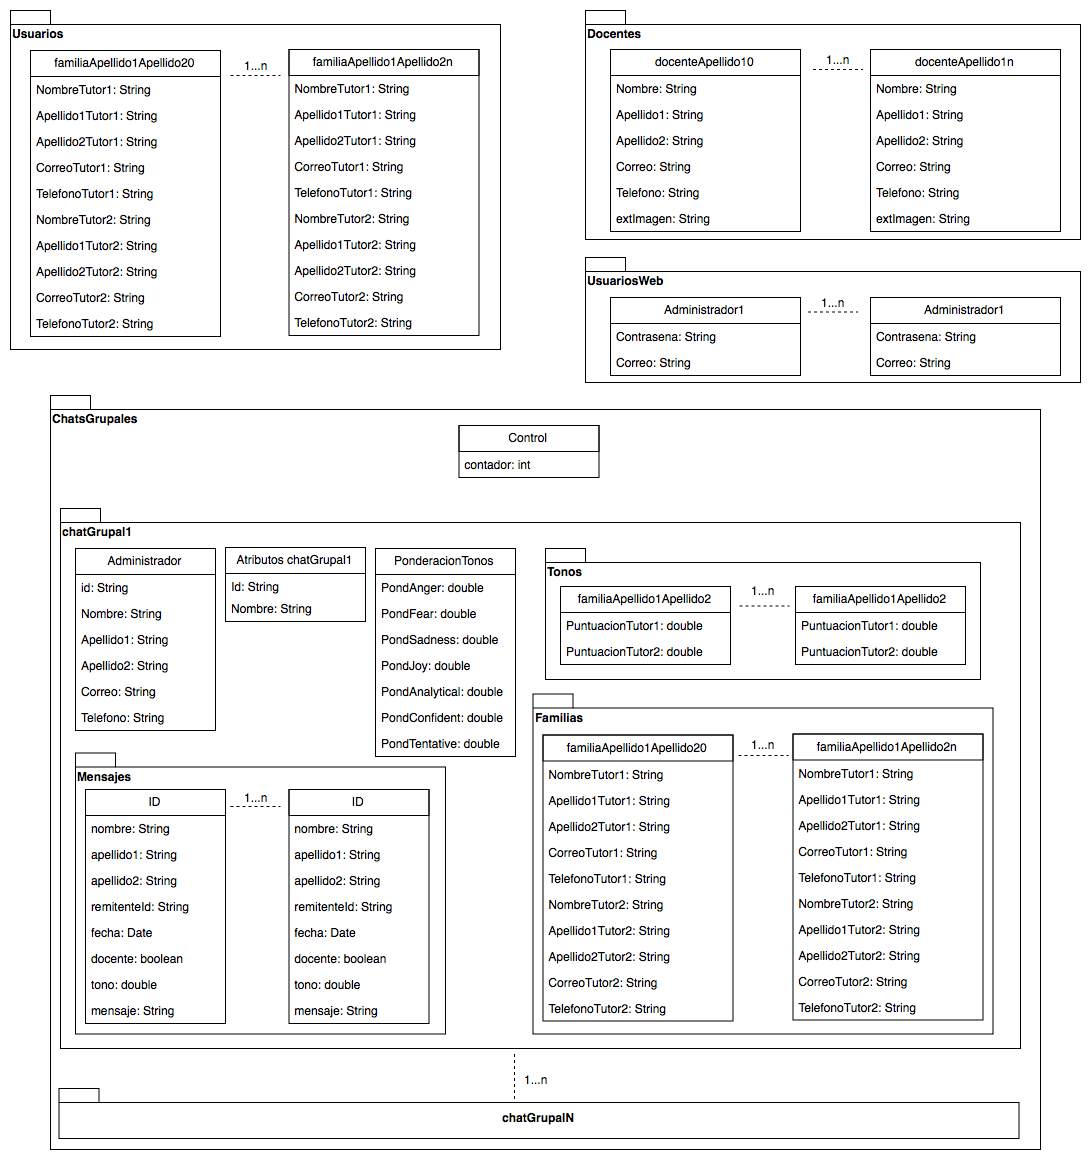
\includegraphics[width=0.9\textwidth]{/BBDDFirestore.png}
		\caption{Diseño de la Base de Datos no Relacional}
		\label{fig:bbddfirestore}
	\end{center}
\end{figure}
